\documentclass[12pt]{article}

\usepackage{sbc-template}
\usepackage{graphicx,url}
\usepackage[utf8]{inputenc}
\usepackage[english]{babel}
\usepackage{color}
%\usepackage{hyperref}

%\usepackage[latin1]{inputenc}  
\sloppy

\title{Code2Algo: A Tool to Recommend Algorithms}

\author{Lucas R. Raggi, Hyago P. Brito, Arthur S. B. de Melo, João M. L. Pereira, \\Baldoino Fonseca, Márcio Ribeiro, Jairo Souza}


\address{Instituto de Computação\\
        Universidade Federal de Alagoas (UFAL) - Maceió - Brasil
  \email{\{lrr, hpb, asbm, jmlp, baldoino, marcio, jrmcs\}@ic.ufal.br}
}

\begin{document} 

\maketitle

\begin{abstract}

    During software development, it is common developers coding algorithms to perform specific tasks. This way, it is essential to understand how to implement them, but it is humanly impossible to remember the whole variety of algorithms, as well as how to implement them correctly. Recent studies provided recommender systems to help developers in software engineering activities. However, none of them focus on making recommendations to assist developers in suggesting algorithms during software development. In this context, we propose Code2Algo, an integrated development tool on the Eclipse platform that receives a code snippet and provides the entire algorithm. Our tool relies on the use of a neural network model trained from extracted incomplete Java code snippets to recommend algorithms, decreasing developers' effort since they will avoid context switching searching algorithms on external resources.
     
     Video: \url{https://youtu.be/sBf-tzyzltE}

\end{abstract}  

\section{Introduction}
  

% Problematic and context
     An algorithm is a finite sequence of computational steps that transform an input into an output aiming at obtaining a solution for a specific type of problem \cite{leiserson2002algoritmos}. In this perspective, developers need to use algorithms to perform different tasks in data structures like search, sorts, split, or other operations to solve problems during software development. However, developers may not know how to implement these solutions because some of these algorithms could not be trivial, reducing the effort to acquire implementations of algorithms through external resources.
   
% Related Works

    Several studies have investigated recommendation systems to assist software engineering tasks using data mining techniques or machine learning approaches. For example, studies suggest recommendations for method invocations and constructors~\cite{Bruch2009}, API calls~\cite{Raychev2014}, code generation~\cite{Vijayaraghavan2017Bayou}, method names~\cite{Alon2018Code2vec}, and generic codes through similar codes~\cite{Luan2018Aroma}. However, none of these studies provided recommendation systems with the possibility of recommending algorithms to assist developers during day-to-day activities.

% Objective
    In this paper, we propose and describe the Code2Algo that consists of an integrated development environment (IDE) tool that consumes an external API which helps developers recommending algorithms during the software development. In addition, this tool can improve developers knowledge and software quality. When using this tool, developers can receive up to three algorithms recommendations based on the incomplete code that they are writing at the moment in the IDE.
    
    The remaining of this paper is structured as follows. Section~\ref{sec:mot} presents the motivation to create our tool. Next, Section~\ref{sec:tool} describes the tool, presenting the main features. In Section~\ref{sec:architecture}, we describe our architecture. Section~\ref{sec:related_work} presents related work, and finally, Section~\ref{sec:conclusion} concludes the study and provides possible futures works.


\section{Motivational Example}
\label{sec:mot}
    
    
    Figure~\ref{fig:binary} presents an incomplete code of \textit{Binary Search} algorithm that finds the position of a target value within a sorted array. In some circumstances, developers can become stuck due not to know how to implement a specific algorithm considering that is expected they have previous experience implementing it.
    
    \begin{figure}[h]
        \centering
        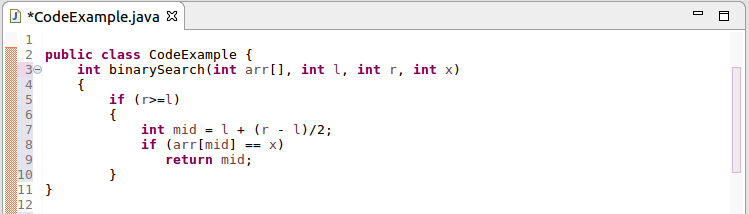
\includegraphics[width=\linewidth]{cbsoft19/figs/binary.png}
        \caption{Example of developer getting stuck}
        \label{fig:binary}
    \end{figure}
    
     To avoid this, developers may check external resources such as documentation or educational repositories that contain various examples of implemented algorithms. However, they would spend extra effort to investigate this outside of their development environment. In addition, various algorithms were created with distinct designs and objectives, so a higher effort is necessary to know all implementations types of them. This is reinforced for novice developers, which have high chances to get stuck when they do not know how to implement a specific algorithm during software development. Therefore, it is necessary the development of tools to recommend algorithms for developers during software engineering tasks to help developers. 
    

\section {Tool}
\label{sec:tool}

    In this section, we present how our tool deals with aforementioned problems and describe the main functionalities. 
    
    Code2Algo~\cite{Code2Algo2019} is an Eclipse plug-in distributed under MIT license that provides support for Java developers during software engineering tasks. It integrates with \textit{Code2Vec} and Eclipse Platform. When using our tool, developers can receive algorithm recommendations during their implementation, i.e., when it is still incomplete. In some cases, even just the algorithm name is enough. In Figure~\ref{fig:recommender}, we present a view of the tool recommending algorithms.  
    
    \begin{figure}[h]
        \centering
        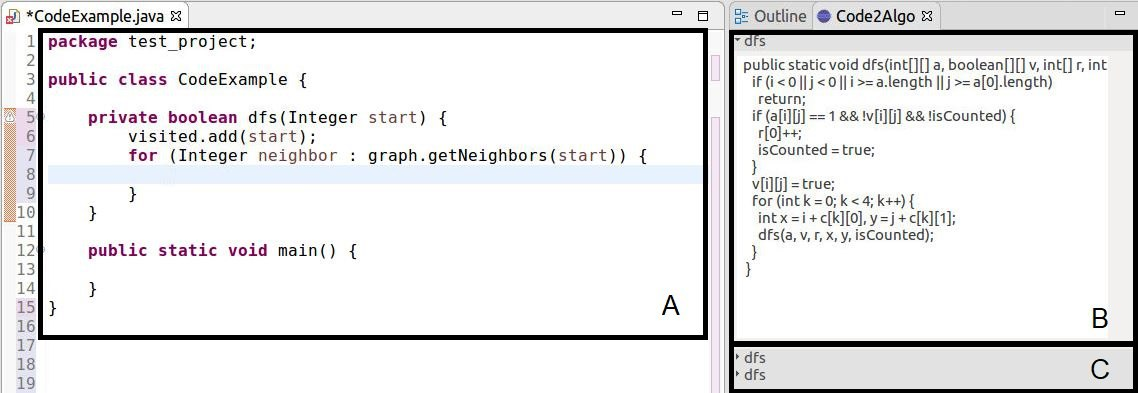
\includegraphics[width=\linewidth]{cbsoft19/figs/Exemplo.jpg}
        \caption{Code2Algo Eclipse plugin recommending up to three algorithms}
        \label{fig:recommender}
    \end{figure}
    
    With our tool, developers can receive recommendations of possible algorithms to finish or complete their code. Every code retrieved is presented in an integrated perspective view with expanding bars, as shown in Figure~\ref{fig:recommender}. To recommend similar algorithms for developers, we consume an API and applied a ranking with three features as detailed in section \ref{sec:architecture}. Next, similar algorithms are identified based on a search in our database and exhibited by the tool. Thus, developers can choose and copy one algorithm to use, or analyze it to develop their own solution using our recommendation provided by Code2Algo as an example.

    Figure~\ref{fig:recommender} presents our plugin recommending \textit{DFS} algorithm to a developer. Part A of the Figure~\ref{fig:recommender} shows an incomplete algorithm under development by a developer. Next, our plugin reads the partial code and send to our API, which reads the request and recommends up to three algorithms. Part B of the  Figure~\ref{fig:recommender} presents the most similar code, while part C exhibits the remaining algorithms ordered by similarity. Finally, the user can copy the code retrieved from this view for use to complete the code under development. 
    
    Besides, Code2Algo also recommend algorithms only with the name of the method, as we can see in Figure~\ref{fig:flow}. Using this feature, a developer provides the name of a specific algorithm \textit{Insertion Sort} and receive recommendations containing possible full algorithms.
    
    \begin{figure}[h]
        \centering
        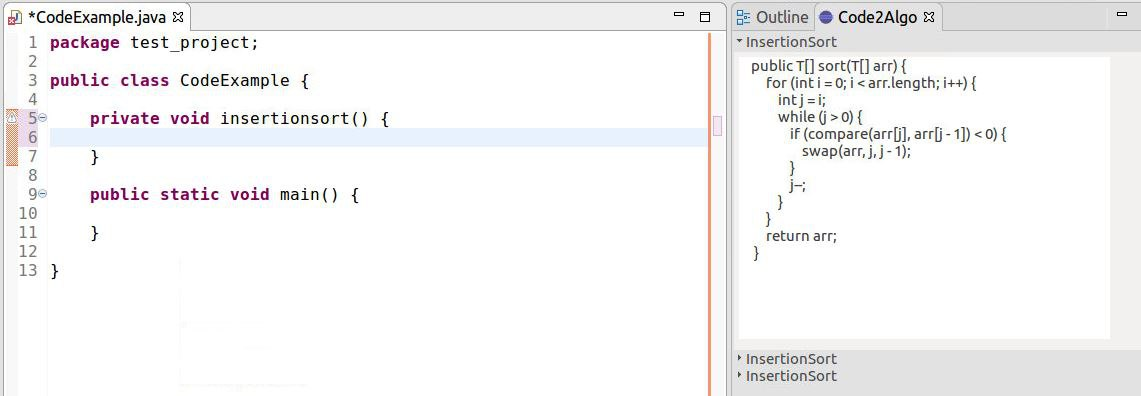
\includegraphics[width=\linewidth]{cbsoft19/figs/capturename.jpg}
        \caption{Algorithm recommendation containing only the method name.}
        \label{fig:flow}
    \end{figure}
    
    %In addition, our plug-in have three ways to operate, the first is based on a complete algorithm developed, can use it to review if its code is the most similar to his code and if its implementation is right. Second, if the developer do not know the implementation of certain algorithm, but knows its name, can try naming a method to retrieve the full algorithm in our tool. Last, if the developer started the algorithm, but got stuck in the middle, he can use our plug-in to finish his code.
    
    \section{Architecture}
    \label{sec:architecture}
    
    In this section, we describe the architecture of our tool that consists on two modules: (i)an Eclipse plug-in that uses an interface based on a perspective view composed of the Eclipse infrastructure using \textit{Java Development Tools} (JDT) library; and (ii) an API with the following components: Code Extractor, Code Identifier, Code Recommender, and a Recommender Database. An overview of the \textit{Code2Vec} architecture is represented in Figure Figure~\ref{fig:api}. 
    
    \begin{figure}[h]
        \centering
        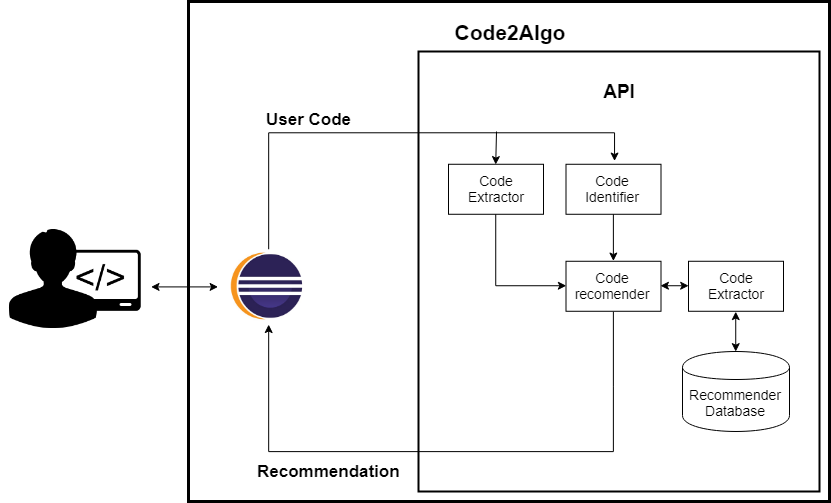
\includegraphics[width=\linewidth]{cbsoft19/figs/Figure2.png}
        \caption{Flow Diagram}
        \label{fig:api}
    \end{figure}

    \textbf{Plugin Interface:} This first step presents the Graphical User Interface(GUI) integrated with the Eclipse IDE. When the developer is typing the code in the IDE editor, our plugin is listening in the background. Then,  the plugin sends a \textit{JSON} object containing the developer's full code and the name of the method. Finally, the API process the request and returns the up to three algorithm recommendations, as shown in Figure~\ref{fig:recommender} Area B and C.
    
    \textbf{Code Identifier:} Contains the trained \textit{Code2Vec} model \cite{Alon2018Code2vec} that is responsible for represents code snippets as a single fixed-length code vector.  With this, is possible to identify a whole algorithm receiving an incomplete snippet or even just the name of the method. To perform this, we use the \textit{Code2Vec} neural model trained with incomplete algorithms using the Java Line Remover obtaining a full algorithm code from selected repositories and removing some lines from it in a way where the code still compilable. This way is possible to collect correct pieces of code to train the \textit{Code2Vec} neural model. Finally, the Code Identifier finds the method in the object and split it to use in our model of Code2Vec, as output we have the name of the algorithm being developed. 
        
    \textbf{Code Extractor:} Consists of a Code2Algo API module, where it picks the code snippet and extract the most relevant information from it such as the return type, number, and type of parameters. It is used in the code received from the user and in the returned codes from our database. 
    
     \textbf{Recommender Database:} A manually selected database composed by algorithms from educational repositories from GitHub, such as \cite{TheAlgotithms} i.e., made by experienced developers.
        
    \textbf{Code Recommender:} Part of API where the ranking is made and based on it, return the code for user. After retrieving all instances of the algorithm identified in the code identifier from our recommender database, the ranking is made based on three parameters which are extracted in Code Extractor from each recommendation candidate and the user code. Each of these metrics receives a score from 0 to 1 based on the similarity between the user code and the candidates, which are algorithms found in our database. Then from the candidates, the best three are selected and returned for the user.
    
    Code2Algo works in the following way. First, the user opens our plug-in and start typing the code. Then, the tool, recognizing that a method is being typed, sends its snippet to the API. The Code Identifier infers which algorithm the user code most closely resembles. Parallel to this, the developer code passes through our Code Extractor to extract the parameters described in the Code Extractor section to use in our ranking.
    
    Moreover, with the identified algorithm the Code Recommender seeks similar algorithms in the Recommender Database, each candidate also passes through the Code Extractor, so the Code Recommender ranks them based on the similarity of the candidates and the user code extracted metrics. Finally, the tool presents the results. These components are described below.
    
   
\section{Related Work}
\label{sec:related_work}
% REVISAR TODOS OS RELACIONADOS PRA VER SE TA CERTO

Several studies have focused on provided software engineering (SE) recommender systems to make recommendations to assist software engineering tasks. These studies use data mining techniques and probabilistic models on various SE artifacts. 

First, \cite{Bruch2009} improve the system of code completions by learning from examples. This algorithm extracts the context of the variable, search for variables used in similar situations and then synthesize method calls recommendations out of these nearest snippets. Moreover, \cite{Raychev2014} used statistical models containing formal source code properties to suggest calls to the APIs. They focus on reducing the problem of code completion to a natural language. To perform this, they extracted sequences of method calls and indexed into a statistic language model permitting to synthesize a code completion.

\cite{Vijayaraghavan2017Bayou} generates code to complete the function that the developer wants to create, it does not use the lines of code that the user is typing, but "draft program" instead, a method with holes and "queries" that are tips you give about the code, what functions it will call, variables to create, etc. 

More recently, \cite{Luan2018Aroma} provided tool that identifies the algorithm using a similar version of \textit{Code2Vec} \cite{Alon2018Code2vec}, that performs a search on a database, select candidates, cluster and intercept them for a good recommendation. Our tool also uses the \textit{Code2Vec} aiming to identify the method name based on a snippet. However, we trained our neural network with incomplete codes, since given an incomplete snippet of code, we recommend similar algorithms.

Such SE recommenders systems provided useful recommendations to help developers during software development. However, our tool differs from the previous works by focusing on recommending different types of algorithms to developers. Thus, developers can focus the effort on other tasks to gain productivity than search on how to implement algorithms in external resources correctly. 

%Code2Algo needs only the lines of code that developer is typing and is restricted to algorithms.

\section{Concluding Remarks and Future Work}
\label{sec:conclusion}

This paper presented Code2Algo, a tool with the intent of helping developers by decreasing the effort needed during the implementation of algorithms in Java. The tool consists of an integrated Eclipse plugin and an API that recommends three most similar algorithms based on the incomplete code of developers during the software development. Also, it is possible to recommend complete algorithms to developers with only the name of them. Our tool is based on \textit{Code2Vec}, a neural model trained with incomplete code snippets, and Base Recommender, a database composed of algorithms from educational repositories. As future work, we intend to implement extension points in the API to integrate to other developers tools, add more features, improve the neural model and Recommender Database with the purpose to identify and recommend more algorithms.

\bibliographystyle{sbc}
\bibliography{sbc-template}

\end{document}
